\documentclass[a4paper,titlepage]{report}



% Packages for graphics and layout
\usepackage{graphicx}
\usepackage[a4paper, margin=1in]{geometry}
\usepackage{titlesec}
\usepackage[dvipsnames]{xcolor}
\usepackage{colortbl}
\usepackage{caption}
\usepackage{calc}
\usepackage{ragged2e}
\usepackage{mdframed}
\usepackage{tikz}
\usepackage{svg}

\usepackage[hidelinks]{hyperref}
\usepackage[margin=1in]{geometry} % Riduzione dei margini

% Packages for math and tables
\usepackage{amsmath}
\usepackage{booktabs}
\usepackage{cellspace} % For adding padding in table cells
\usepackage{tabularx}
\usepackage{multirow}
\usepackage{array}
\usepackage{longtable}

% Packages for references and the table of contents
\usepackage{hyperref} % For links in the table of contents
\usepackage{tocbibind} % To include the table of contents in the table of contents

% Packages for code
\usepackage{listings}
\usepackage{courier} % Font for code
\usepackage{fancyvrb}
\usepackage{lipsum} % For dummy text

% Remove paragraph indentation and add space between paragraphs
\usepackage{parskip}  
\usepackage{algorithm}
\usepackage{algpseudocode}

% Set the table format for the combiner and in mapper part
\setlength{\extrarowheight}{5pt} % Extra vertical padding
\setlength{\tabcolsep}{10pt} % Extra horizontal padding

% Define custom colors
\definecolor{myBlue}{rgb}{0.0745, 0.2157, 0.4118}
\definecolor{myLightBlue}{rgb}{0, 0.5647, 0.5843}
\definecolor{myGray}{RGB}{192,197,206}
\definecolor{myPurple}{rgb}{0.5, 0.0, 0.5} % Esempio di colore viola
\definecolor{myLightPurple}{HTML}{CC0066} % Esempio di colore viola chiaro
\definecolor{jsonString}{HTML}{111258}
\definecolor{numb}{RGB}{255,0,0}
\definecolor{punct}{RGB}{0,0,255}
\definecolor{delim}{RGB}{20,105,176}
\definecolor{comment}{RGB}{0,128,0}
\definecolor{string}{RGB}{163,21,21}
\definecolor{keyword}{RGB}{0,0,255}
\definecolor{darkgreen}{rgb}{0,0.5,0}
\definecolor{java_keyword}{HTML}{BF9B30}
\definecolor{java_comment}{HTML}{0000FF}
\definecolor{mybackgroundcolor}{RGB}{240, 240, 240} % Light gray background
\definecolor{black}{RGB}{0, 0, 0} % Define black color
\definecolor{jsondoc}{HTML}{C4E3E8}
\definecolor{red}{HTML}{8F1D39}
\definecolor{white}{RGB}{255,255,255} % Define white color



% Define shades of green
\definecolor{myDarkGreen}{RGB}{0, 100, 0} % Dark green
\definecolor{myGreen}{RGB}{0, 128, 0} % Medium green
\definecolor{myLightGreen}{RGB}{144, 238, 144} % Light green




% Configuration for section titles
\titleformat{\section}[hang]{\Large\bfseries\color{myDarkGreen}}{}{0px}{}[\titlerule]
\titleformat{\subsection}[hang]{\large\bfseries\color{myGreen}}{}{0em}{}
\titleformat{\subsubsection}[hang]{\bfseries\color{myLightGreen}}{}{0em}{}

% Configuration for chapter titles
\titleformat{\chapter}[display]
  {\normalfont\Large\bfseries\color{myGreen}}{}{-80pt}{\LARGE}
\renewcommand{\chaptername}{} % Remove the word "Chapter" and the number from the title
\setcounter{tocdepth}{1} % Include only chapters and sections in the table of contents

% Style for code
\lstdefinestyle{mystyle}{
    language=Java,
    backgroundcolor=\color{mybackgroundcolor}, % Background color
    commentstyle=\color{darkgreen},
    keywordstyle=\color{blue},
    numberstyle=\tiny\color{gray},
    stringstyle=\color{orange},
    basicstyle=\ttfamily\footnotesize,
    framesep=10pt, % padding between frame and text
    xleftmargin=10pt, % left margin
    xrightmargin=10pt, % right margin
    aboveskip=10pt, % Top padding
    belowskip=10pt, % Bottom padding
    breakatwhitespace=false,         
    breaklines=true,                 
    captionpos=b,                    
    keepspaces=true,                 
    numbers=left,                    
    numbersep=5pt,                  
    showspaces=false,                
    showstringspaces=false,
    showtabs=false,                  
    tabsize=2
}

\lstdefinestyle{mystyle}{
    backgroundcolor=\color{white},   % background color
    basicstyle=\ttfamily\footnotesize, % basic font style
    breaklines=true,                  % line breaking
    captionpos=b,                     % caption position
    numbers=left,                     % line numbers on the left
    numbersep=5pt,                    % distance of line numbers from the code
    showspaces=false,                % don't show spaces
    showstringspaces=false,          % don't show string spaces
    showtabs=false,                  % don't show tabs
    tabsize=2                         % tab size
}

\lstset{style=mystyle}

\lstdefinestyle{pythonstyle}{
    language=Python,
    basicstyle=\ttfamily\footnotesize,
    breaklines=true,
    captionpos=b,
    numbers=left,
    numbersep=5pt,
    showspaces=false,
    showstringspaces=false,
    showtabs=false,
    tabsize=4
}

\lstset{style=pythonstyle}

\begin{document}

\begin{titlepage}
    \centering
    \vspace*{\fill}
    {\LARGE \textbf{UNIVERSITY OF PISA}}\\[0.5cm]
    \begin{figure}[h]
        \centering
        
\includegraphics[width=0.4\textwidth]{media/university-of-Pisa-logo.jpg}
    \end{figure}
    {\Large \textit{Artificial Intelligence and Data Engineering}}\\[1.5cm]
    {\LARGE \textbf{Internet of Things}}\\[1cm]
    {\Large \textit{SeedBot: Automated Sowing Device}}\\[2cm]
    
    {\large \textbf{Francesco Nocella, Noemi Cherchi}}\\[0.5cm]
    {\large Academic Year 2023/2024}
    \vspace*{\fill}
\end{titlepage}

\tableofcontents

\chapter{Introduction}

SeedBot is an automated system designed for agricultural sowing. It uses a network of wireless sensors to monitor soil conditions and control the seed distribution mechanism, improving efficiency and reducing manual labor. Using a pre-trained machine learning model, SeedBot can determine the most suitable crop for a specific plot of land.

\subsection{Use Case}
The agricultural sector plays a crucial role in the industry, specifically when considering large-scale food production, which requires high efficiency, a strict quality check and optimized comunication among the different phases of the production process. However, traditional farming methods are labor-intensive and often inefficient. 
In the contest of smart industries, the use of IoT devices and machine learning algorithms can significantly improve agricultural processes.\\


SeedBot aims to address these challenges by automating the sowing process, optimizing seed distribution based on real-time soil data, and reducing the need for manual intervention. This allows the sowing to happen in in optimal conditions, minimazing errors and the waste of resources.\\

SeedBot receives real-time data from various sensors, including nitrogen, phosphorus, and potassium (NPK) levels, soil moisture, pH, and air temperature. This data is used to determine the best seed type for the soil conditions and control the seed distribution mechanism accordingly. The position and the results of the sowing are then sent to a central server for monitoring and analysis, which allows farmers to correct anomalies and optimize the sowing process.\\

This means that SeedBot allows to reduce operational costs and production time, helping to make the farms more competitive on the global market.
\chapter{System Architecture and Load Distribution}

In this project, six nRF52840 devices are employed to implement the testing of a fully automated sowing system. These devices are specifically organized into roles for sensors and actuators to ensure efficient communication, data collection, and actuation. The system is designed to optimize task distribution across devices while maintaining scalability and performance.

The system architecture is composed of the following elements


\begin{figure}[H]
    \centering
    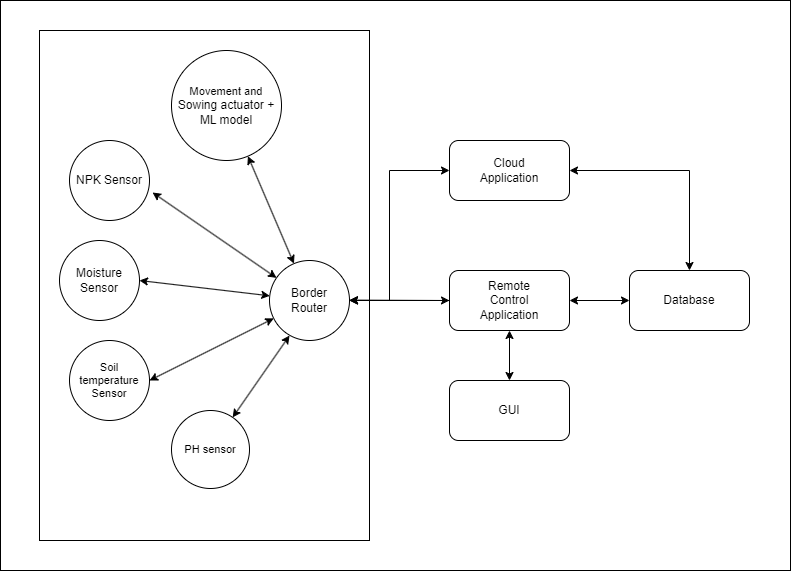
\includegraphics[width=0.7\textwidth]{media/IoT_architecture.png}
    \caption{SeedBot Architecture}
    \label{fig:SeedBot Architecture}
\end{figure}

\begin{itemize} 
    \item \textbf{Border Router:} 
    \begin{itemize} 
        \item Acts as the central communication hub, managing all data exchanges between sensors, actuators, and cloud or remote applications using the CoAP protocol, ensuring efficient data flow. 
    \end{itemize} 
    \item \textbf{Sensors:} 
    \begin{itemize} 
        \item \textbf{NPK Sensor:} Measures the soil's nitrogen, phosphorus, and potassium levels. 
        \item \textbf{Moisture Sensor:} Monitors soil moisture levels to ensure optimal growing conditions. 
        \item \textbf{PH Sensor:} Measures the soil pH levels, helping optimize the sowing conditions based on acidity or alkalinity. 
        \item \textbf{Temperature Sensor:} Collects soil temperature data to help in seed germination analysis. 
    \end{itemize} \item \textbf{Actuator:} 
    \begin{itemize} \item \textbf{Movement and Sowing Actuator:} Controls the robot’s movement and seed distribution. Decisions are made based on input from the machine learning model to ensure efficient sowing. 
    \end{itemize} \item \textbf{Applications:} 
    \begin{itemize} \item \textbf{Cloud Application:} Handles the storage and processing of sensor data in a central database. 
        \item \textbf{Remote Control Application:} Provides a graphical user interface that allows users to remotely control the system and monitor real-time data. 
    \end{itemize} 
\end{itemize}

This balanced division of labor ensures that the workload is effectively shared among the devices, allowing the system to operate smoothly and in real-time while minimizing latency and maximizing resource utilization.
\chapter{Machine Learning Model}

The initial dataset was taken from \href{https://www.kaggle.com/code/mdshariaremonshaikat/optimizing-agricultural-production-with-7-ml-model/input}{kaggle}. The dataset contains information about different crops and their requirements in terms of soil conditions, such as nitrogen, phosphorus, and potassium levels, soil moisture, pH and temperature. 
The types of crop include: rice, chickpea, kidney beans, lentil, pomegranate, banana, mango, papaya, etc.\\
The dataset was preprocessed to remove missing values and was then split into training and testing sets.\\
To create the model, multiple machine learning methods were used and evaluated for their accuracy in predicting crop suitability. In particular, classifiers like Logistic Regression, Random Forest, Gradient Boosting, Support Vector Machines (SVM), Naive Bayes, Decision Tree, and K-Nearest Neighbors (KNN) were used.\\
The final model was trained using the Decision Tree algorithm, which achieved an accuracy of 98.64\% on the test set.
The Decision Tree algorithm was chosen not only for its high accuracy but also for its interpretability, which is crucial in agricultural applications where understanding the decision-making process is as important as the prediction itself. The tree-based structure of this algorithm allows for clear visualization of how specific soil conditions lead to the recommendation of certain crops, making it easier for end-users, such as farmers, to trust and follow the model's advice.
The model was exported using the Python library \texttt{emlearn} and integrated into the SeedBot system to make real-time crop recommendations based on soil conditions, providing a practical tool to optimize agricultural production.


\chapter{Code and Software}

The code for SeedBot is written in C and Python. The nRF52840 devices run the C code, while the cloud and remote applications are written in Python. The code is available on GitHub at the following \href {https://github.com/}{link}.



\subsection{C Code}



The actuator code is responsible for controlling the movement and seed distribution of the robot. It receives commands from the machine learning model and executes them accordingly.


\textbf{Actuator Workflow}

\begin{enumerate}
    \item \textit{Initialization and Registration:}
    \begin{itemize}
        \item The first step involves registering with the CoAP server. This process includes sending a\\
         registration request to the server with the actuator's name and its IPv6 address. The\\
         registration can be attempted 5 times.
    \end{itemize}
    
    \item \textit{Discovery of Sensor IP Addresses:}
    \begin{itemize}
        \item After the registration, a CoAP discovery request is performed to find the IP addresses of the sensors: \texttt{npk}, \texttt{ph}, \texttt{moisture}, and \texttt{temperature}. Each answer is analyzed to extract and store the IP addresses of the sensors.
    \end{itemize}
    
    \item \textit{Retrieving Sensor Data and Determining the Seeding Type:}
    \begin{itemize}
        \item Once the command is received, a CoAP GET request is performed to collect data from the sensors.
        \item Machine learning algorithms are used to analyze the collected sensor data and decide the type of seed to use based on the gathered information.
    \end{itemize}
    
    \item \textit{Simulating the Seeding Operation:}
    \begin{itemize}
        \item The seeding operation is simulated by introducing a delay that represents the time taken for seeding.
        \item A yellow LED is turned on to indicate that the seeding operation is in progress.
        \item The actuator can start or pause the movement of the robot based on the pressing of the button.
    \end{itemize}
    
    \item \textit{Updating the Central CoAP Server:}
    \begin{itemize}
        \item A CoAP message is sent to the central server with details of the seeding operation, including the type of seed used, the current row and column, and the sensor values.
    \end{itemize}
    
    \item \textit{Restarting Until the Field is Completely Sowed:}
    \begin{itemize}
        \item The process loops back to step 3 until the entire field is completely sowed.
    \end{itemize}
    
\end{enumerate}

\newpage


The sensors code reads the generated data and sends it to the border router for processing.


\textbf{Sensors Workflow}

\begin{enumerate}
    \item \textit{Initialization and Registration:}
    \begin{itemize}
        \item Each sensor is initialized by registering with the central CoAP server. The sensor's name and its IPv6 address is sent to the server.
    \end{itemize}

    \item \textit{Activation of Sensor Resources:}
    \begin{itemize}
        \item Once registration is successful, the sensor activates its corresponding resources (e.g., moisture, pH, NPK, temperature) to be available for CoAP requests.
    \end{itemize}
    
    \item \textit{Data Simulation:}
    \begin{itemize}
        \item Each sensor simulates data readings based on predefined statistical distributions. The values are constrained to realistic ranges for each parameter using a normal distribution with specified mean and standard deviation:
        \begin{itemize}
            \item \textbf{Moisture Sensor:} The values are bounded between 0 and 100.
            \item \textbf{pH Sensor:}The values are constrained between 3.5 and 10.
            \item \textbf{NPK Sensor:} The values are bounded by realistic agricultural ranges.
            \item \textbf{Temperature Sensor:} The values are bounded between 8.8°C and 43.7°C.
        \end{itemize}
    \end{itemize}
    
    \item \textit{Handling CoAP GET Requests:}
    \begin{itemize}
        \item Each sensor responds to CoAP GET requests. It the simulated data and returns it in a JSON format within the CoAP response.
    \end{itemize}

    \item \textit{Retry Mechanism for Registration:}
    \begin{itemize}
        \item If the initial registration attempt fails, the sensor will retry registration for a predefined number of times, introducing a delay between each attempt.
    \end{itemize}

    \item \textit{Operational Loop:}
    \begin{itemize}
        \item Once registered, the sensor enters a loop where it continues to respond to incoming CoAP requests while maintaining its simulated data. The process continues indefinitely as long as the sensor is active.
    \end{itemize}
    
\end{enumerate}


\newpage

\subsection{Python Code}


The Python code is responsible for managing the cloud and remote applications. The cloud application stores data collected from the sensors in a database, while the remote control application allows users to interact with the system via a graphical interface.\\

There are two comunication protocols: HTTP (through the Flask library) and CoAP (Constrained Application Protocol). The HTTP protocol is used for the cloud application, while the CoAP protocol is used by the remote control application.\\
Flask is used to create a RESTful API that allows users to interact with the system. Through the graphical interface, users can initiate, pause and completely stop the sowing process. The API provides endpoints for registering sensors, receiving sensor data, and storing it in the database. Additionally, it handles communication with the actuators via CoAP to manage the different stages of the sowing process, including start, idle, and stop.\\

The server CoAP is used to manage the communication between the sensors and the actuators. It is responsible for registering sensors, receiving sensor data, and sending commands to the actuators. It provides endpoints for sensor registration, data retrieval, and actuator control allowing the system to respond in real-time to the commands sent from the Flask-based user interface.



\textbf{Workflow}
\begin{enumerate}
    \item \textit{Sensor Registration:} 
    \begin{itemize}
        \item The CoAP server receives registration requests from the sensors and stores their information in the database using the \texttt{db\_manager\_mysql} module. Each sensor is assigned a unique identifier and its status is tracked in the database. The server confirms the registration and handles any registration errors.
    \end{itemize}
    
    \item \textit{Data Retrieval:}
    \begin{itemize}
        \item The CoAP server responds to CoAP GET requests from sensors or actuators. The data is read from the database.
    \end{itemize}

    \item \textit{Sensor Data Handling:} 
    \begin{itemize}
        \item Sensors periodically send data (e.g., soil moisture, temperature) to the CoAP server via POST requests. The server processes these requests, extracts the data, and stores it in the database.
    \end{itemize}
    
    \item \textit{Actuator Control:} 
    \begin{itemize}
        \item The cloud application, potentially driven by machine learning models, determines the necessary actions (e.g., sowing seeds) and sends commands to the CoAP server via HTTP.
        \item The CoAP server then translates these commands into CoAP POST requests that are sent to the appropriate actuators. 
    \end{itemize}
    
    \item \textit{Sowing Process Management:} 
    \begin{itemize}
        \item The cloud application monitors and manages the sowing process by sending start, idle, or stop commands to the actuators via the CoAP server. 
    \end{itemize}
    
    \item \textit{Database Interaction:}
    \begin{itemize}
        \item Both \texttt{app.py} and \texttt{coap\_server.py} interact with the MySQL database through the\\
        \texttt{db\_manager\_mysql.py} module. This module handles all CRUD operations, ensuring that sensor data, actuator statuses, and other critical information are properly stored and retrieved as needed.
    \end{itemize}
    
    \item \textit{Response Handling and Logging:} 
    \begin{itemize}
        \item The system logs all key events, such as sensor registrations, data retrievals, and actuator commands, for monitoring and debugging purposes. 
    \end{itemize}
\end{enumerate}


\chapter{Grafana}

Grafana is an open-source platform for monitoring and observability. It allows you to query, visualize, alert on, and understand your metrics no matter where they are stored. In this project, Grafana is used to visualize the database data and analytics.



\begin{figure} [H]
    \centering
    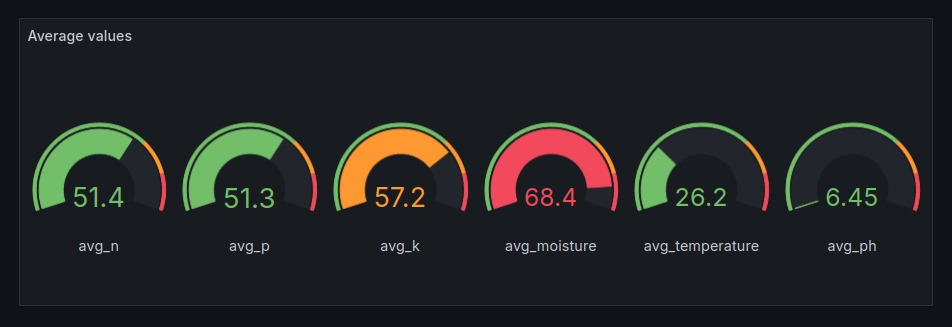
\includegraphics[width=0.8\textwidth]{media/grafana_4.jpg}
    \caption{Graphic showing the average of plant growth parameters such as temperature, pH, humidity, and nutrients (N, P, K) for each field.}
    \label{fig:grafana}
\end{figure}


\begin{figure} [H]
    \centering
    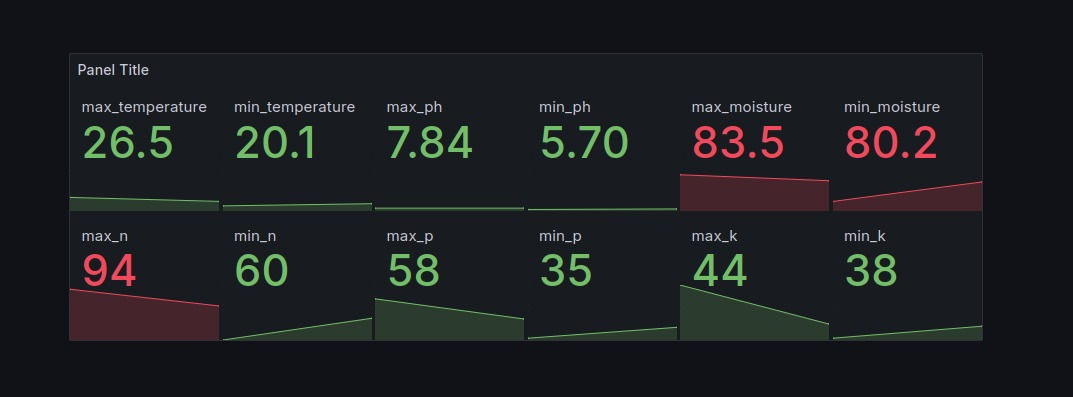
\includegraphics[width=0.8\textwidth]{media/grafana_3.jpg}
    \caption{Graphic showing maximum and minimum statistics for various plant growth parameters such as temperature, pH, humidity, and nutrients (N, P, K), grouped by sowing state.}
    \label{fig:grafana}
\end{figure}
\chapter{Conclusion}


\subsection{Future Implementation}

In the future, SeedBot could be improved by including:

\begin{itemize}
    \item \textbf{Advanced Machine Learning Algorithms:} To further optimize seed distribution and adapt to various weather and soil conditions, enabling predictive analytics for sowing times and crop yields.
    \item \textbf{Advanced Remote User Interface:} Using platforms like Grafana to monitor sensor data in real-time and provide a more interactive user interface, allowing users to set thresholds for various parameters (e.g., soil moisture, pH levels) and receive automated alerts.
    \item \textbf{Integration with Irrigation and Nutrition Systems:} To provide a complete crop management system that includes not only sowing but also irrigation and plant nutrition, with intelligent scheduling based on environmental data.
    \item \textbf{Energy Efficiency and Sustainability Improvements:} Introducing low-power modes and energy-efficient protocols to extend the battery life of the devices and explore the use of renewable energy sources like solar panels to power the system in the field.
    \item \textbf{Blockchain for Data Integrity:} Utilizing blockchain technology to ensure the integrity of data collected from the sensors, providing transparent and tamper-proof records of farming activities, useful for certifications and traceability.
\end{itemize}



\subsection{Conclusion}

This project has demonstrated that handling advanced technologies, such as IoT devices and machine learning, can greatly improve the agricultural sector. The power of nRF52840 devices and the CoAP protocol helps to utilize the resources in an efficient and precise way.
Automating key processes like soil monitoring and seed sowing, means that the need for manual intervention reduces significantly. This approach has the potential to revolutionize farming practices, making them more sustainable and productive. The successful implementation of this system paves the way for further innovations in smart agriculture, ultimately contributing to a more efficient and data-driven approach to farming.



\end{document}
